\documentclass[preprint, 3p,
authoryear]{elsarticle} %review=doublespace preprint=single 5p=2 column
%%% Begin My package additions %%%%%%%%%%%%%%%%%%%

\usepackage[hyphens]{url}

  \journal{Ecology Letters} % Sets Journal name

\usepackage{lineno} % add
  \linenumbers % turns line numbering on

\usepackage{graphicx}
%%%%%%%%%%%%%%%% end my additions to header

\usepackage[T1]{fontenc}
\usepackage{lmodern}
\usepackage{amssymb,amsmath}
\usepackage{ifxetex,ifluatex}
\usepackage{fixltx2e} % provides \textsubscript
% use upquote if available, for straight quotes in verbatim environments
\IfFileExists{upquote.sty}{\usepackage{upquote}}{}
\ifnum 0\ifxetex 1\fi\ifluatex 1\fi=0 % if pdftex
  \usepackage[utf8]{inputenc}
\else % if luatex or xelatex
  \usepackage{fontspec}
  \ifxetex
    \usepackage{xltxtra,xunicode}
  \fi
  \defaultfontfeatures{Mapping=tex-text,Scale=MatchLowercase}
  \newcommand{\euro}{€}
\fi
% use microtype if available
\IfFileExists{microtype.sty}{\usepackage{microtype}}{}
\usepackage[]{natbib}
\bibliographystyle{plainnat}

\usepackage{graphicx}
\ifxetex
  \usepackage[setpagesize=false, % page size defined by xetex
              unicode=false, % unicode breaks when used with xetex
              xetex]{hyperref}
\else
  \usepackage[unicode=true]{hyperref}
\fi
\hypersetup{breaklinks=true,
            bookmarks=true,
            pdfauthor={},
            pdftitle={Impacts of experimental warming on tundra plant flowering phenology},
            colorlinks=false,
            urlcolor=blue,
            linkcolor=magenta,
            pdfborder={0 0 0}}

\setcounter{secnumdepth}{5}
% Pandoc toggle for numbering sections (defaults to be off)


% tightlist command for lists without linebreak
\providecommand{\tightlist}{%
  \setlength{\itemsep}{0pt}\setlength{\parskip}{0pt}}



\usepackage{float}



\begin{document}


\begin{frontmatter}

  \title{Impacts of experimental warming on tundra plant flowering
phenology}
    \author[The University of British Columbia]{Nicola F. Rammell%
  \corref{cor1}%
  \fnref{1}}
   \ead{rammell@student.ubc.ca} 
      \affiliation[Department of Geography]{Department of Geography -
The University of British Columbia}
    \cortext[cor1]{Corresponding author}
  
  \begin{abstract}
  Climate warming is driving rapid shifts in tundra vegetation.
  \end{abstract}
    \begin{keyword}
    phenology \sep climate change \sep alpine \sep tundra \sep 
    plant ecology
  \end{keyword}
  
 \end{frontmatter}

\hypertarget{introduction}{%
\section{Introduction}\label{introduction}}

Climate warming is driving rapid shifts in tundra vegetation. This study
uses data from Carbognani et al., 2018, accessed from Dryad, to plot
phenological development of three alpine plant species as a function of
air temperature. In this study, temperature was manipulated using
experimental warming to simulate climate warming of 1-3 degrees C. Data
was collected in the Italian Alps during the 2010-2014 growing seasons.
An improved understanding of how species will react to warming is
imperative in tundra environments where climate warming is driving rapid
shifts in vegetation.

\hypertarget{methods}{%
\section{Methods}\label{methods}}

Researchers collected data on three different plant species from
2005-2007 in the Italian Alps. Air temperature was manipulated
experimentally and phenophases were recorded for \emph{Cardamine
alpina}, \emph{Leucanthemopsis alpina}, and \emph{Veronica alpina}
throughout the growing seasons. In this paper, I plot the data by
species.

\hypertarget{results}{%
\section{Results}\label{results}}

The phenological development of \emph{Cardamine alpina},
\emph{Leucanthemopsis alpina}, and \emph{Veronica alpina} all increased
with temperature (Fig. 1)

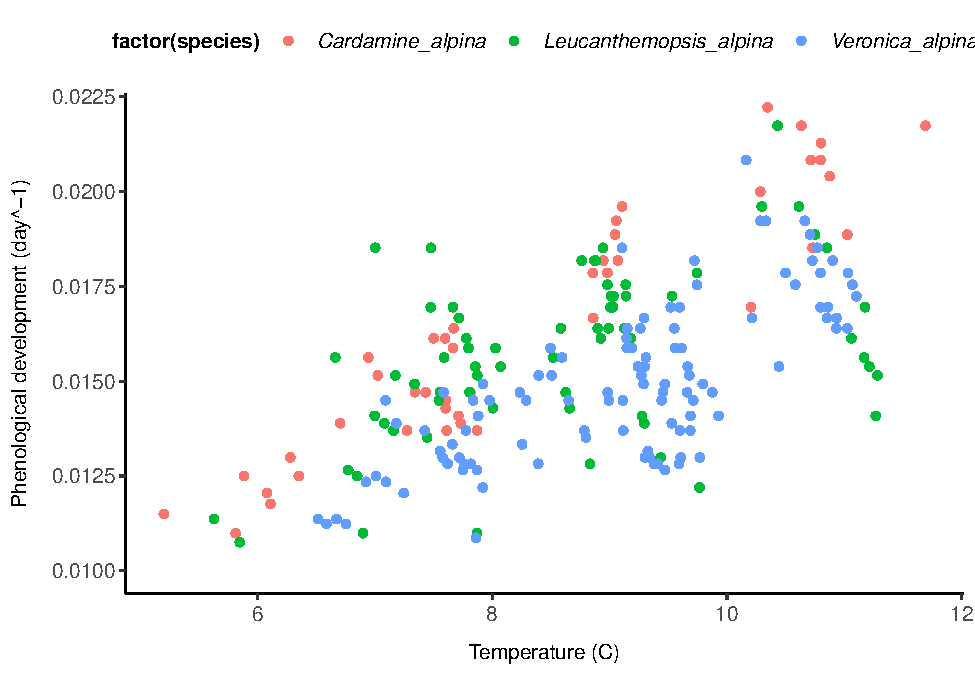
\includegraphics{manuscript_files/figure-latex/unnamed-chunk-1-1.pdf}
\textbf{Figure 1.} Phenological development as a function of temperature
for three alpine species, Cardamine alpina, Leucanthemopsis alpina, and
Veronica alpina.

\hypertarget{discussion}{%
\section{Discussion}\label{discussion}}

Species specific responses.

\hypertarget{conclusions}{%
\section{Conclusions}\label{conclusions}}

This is important for reasons.

\hypertarget{acknowledgements}{%
\section{Acknowledgements}\label{acknowledgements}}

CIEE team.

\hypertarget{references}{%
\section{References}\label{references}}

\textless insert references from .bib file\textgreater{}

\bibliography{references.bib}


\end{document}
